%!TEX root = Report.tex

% Overvej at kalde dette afsnit "Experimentation" eller "Testing"
% 
% vis hvornår det virker og hvornår det ikke virker. 
% Se at det virker når vi regnede med at det virkede.
% 
% Hvad tester vi?
% Hvordan tester vi det?
% Virkede det efter hensigten?
% Hvorfor/hvorfor ikke?
% Er der nok testing?
% Hvordan kan man lave mere testing?
% Er der andre måder vi kunne have testet på? (fordele og ulemper ved det)

%---->>>Vi mangler noget om hvor lang tid af gangen vi kan tracke!

\subsection{Testing the tracking software with real ants}
\label{testing}

Having solved the problem of finding an ant on a single image and integrated our software with the XY-plotter and camera, this section focus on testing how the integrated solution works with a video feed of an ant running arond in a controlled environment.\\

The test were performed in a ordinary office environment, with the plotter placed on a table. The room were only lit by daylight, and we used the setup explained in section (REF HANDLING ANTS), with a petridish filled with ground material surround by water, as can be seen in Figure (INSERT FIGURE WITH IMAGE OF SETUP). According to our experimentation in (INSERT REF TO EXPERIMENTATION) we painted our ant with a white color to have the best possible color for tracking. The goal of this test, is to test ant tracking in an environment that is as close to a real environment as possible, and yet by still be in a controlled environment where we could track the ant.corollary\\


In the following we will show several results of running the software, both where the tracking works as intented, but also situations where the software does not work. We will end this section with a summary of the challenges presented by this real-time testing and suggest possible solutions to the problems and an overall evaluation of how the software together with the plotter an camera performs. We will also comment on the important observations done during testing.\\

We will begin by showing several images from the test where the software tracking works. Examples can be seen in Figure \ref{fig:ant_tracking}. We are showin both the final thresholded image, as well as the original image. For this test, following values were used $\alpha = 2.0$ and $T = 240$.\\

\begin{figure}
        \centering
        \begin{subfigure}[b]{0.35\textwidth}
                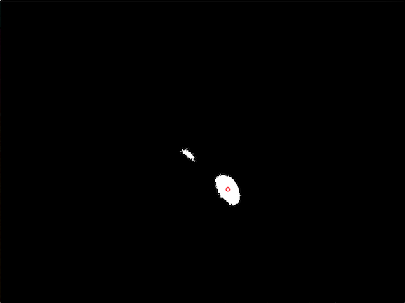
\includegraphics[scale = 0.3]{img/good1t}
                \caption{}
        \end{subfigure}
		\quad
        \begin{subfigure}[b]{0.35\textwidth}
                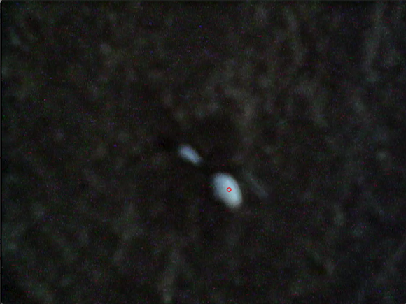
\includegraphics[scale = 0.3]{img/good1}
                \caption{}
        \end{subfigure} \hfill \\ \mbox{}\\
        \begin{subfigure}[b]{0.35\textwidth}
                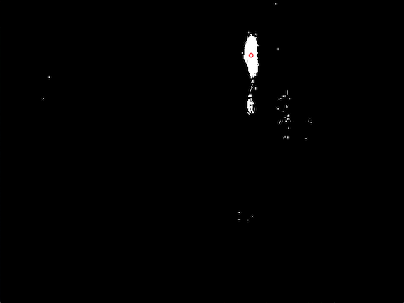
\includegraphics[scale = 0.3]{img/good2t}
                \caption{}
        \end{subfigure}
		\quad
        \begin{subfigure}[b]{0.35\textwidth}
                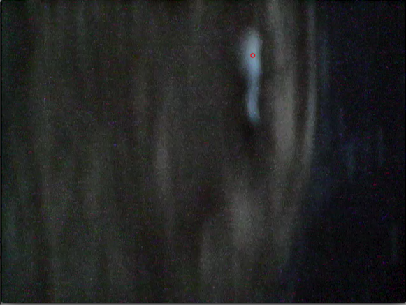
\includegraphics[scale = 0.3]{img/good2}
                \caption{}
        \end{subfigure}\hfill \\ \mbox{}\\
        \begin{subfigure}[b]{0.35\textwidth}
                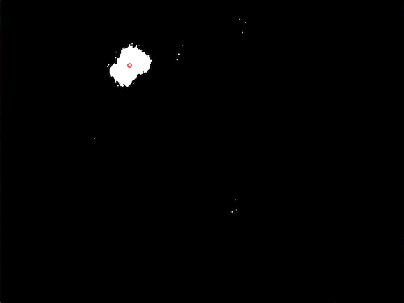
\includegraphics[scale = 0.3]{img/good3t}
                \caption{}
        \end{subfigure}
		\quad
        \begin{subfigure}[b]{0.35\textwidth}
                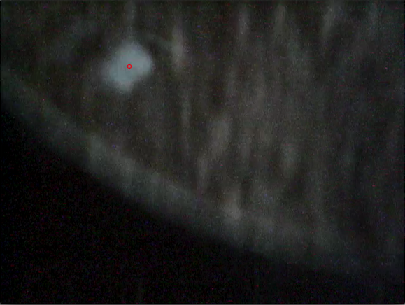
\includegraphics[scale = 0.3]{img/good3}
                \caption{}
        \end{subfigure}\\ \mbox{}\\
        \begin{subfigure}[b]{0.35\textwidth}
                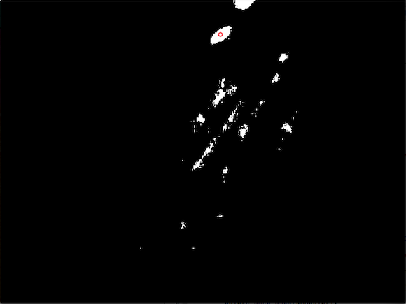
\includegraphics[scale = 0.3]{img/good4t}
                \caption{}
        \end{subfigure}
		\quad
        \begin{subfigure}[b]{0.35\textwidth}
                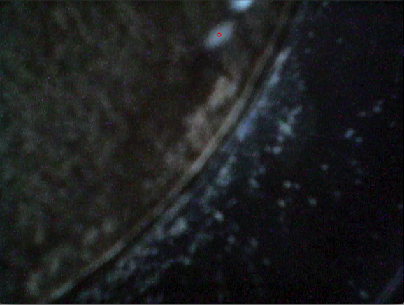
\includegraphics[scale = 0.3]{img/good4}
                \caption{}
        \end{subfigure}
		\caption{Examples of real-time ant tracking.}
		\label{fig:ant_tracking}
\end{figure}

We can see from the images in Figure \ref{fig:ant_tracking} that the software is able to handle different situations where a) the image is very blurry, b) there a noise in the thresholded images and c) where the ant is clearly visible. In general, we can say that it is possible to track the ant in situations where it is distinguishable from anything else in the image, or when it is the largest object present after image processing. However our tests also showed that at times we were unable to track the ant as shown in Figure \ref{fig:ant_fail}.\\

\begin{figure}
        \centering
        \begin{subfigure}[b]{0.35\textwidth}
                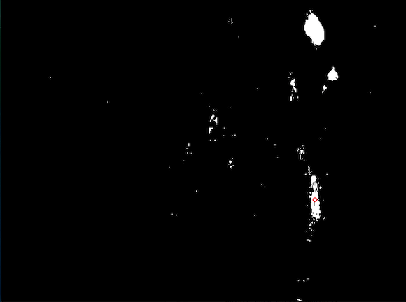
\includegraphics[scale = 0.3]{img/bad1t}
                \caption{}
        \end{subfigure}
		\quad
        \begin{subfigure}[b]{0.35\textwidth}
                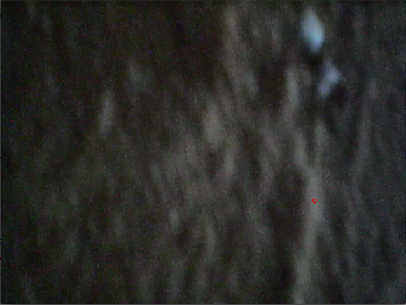
\includegraphics[scale = 0.3]{img/bad1}
                \caption{}
        \end{subfigure} \hfill \\ \mbox{}\\
        \begin{subfigure}[b]{0.35\textwidth}
                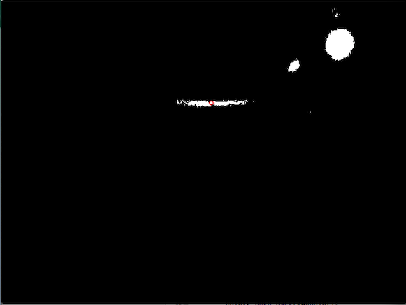
\includegraphics[scale = 0.3]{img/bad2t}
                \caption{}
        \end{subfigure}
		\quad
        \begin{subfigure}[b]{0.35\textwidth}
                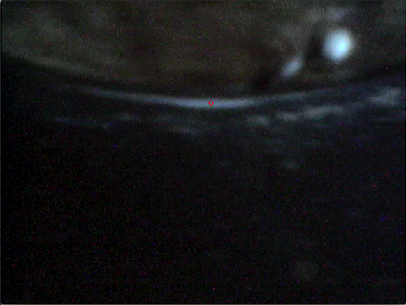
\includegraphics[scale = 0.3]{img/bad2}
                \caption{}
        \end{subfigure}\hfill \\ \mbox{}\\
        \begin{subfigure}[b]{0.35\textwidth}
                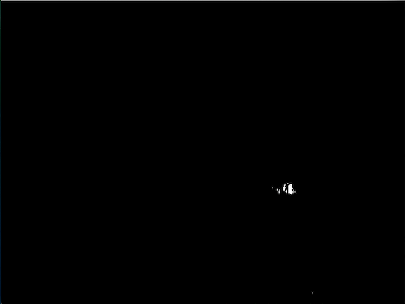
\includegraphics[scale = 0.3]{img/bad3t}
                \caption{}
        \end{subfigure}
		\quad
        \begin{subfigure}[b]{0.35\textwidth}
                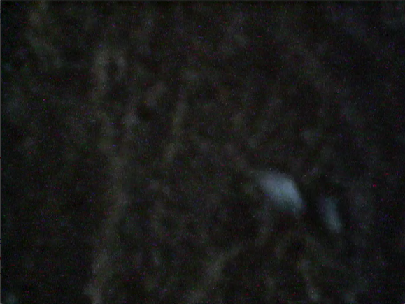
\includegraphics[scale = 0.3]{img/bad3}
                \caption{}
        \end{subfigure}\\ \mbox{}\\
        \begin{subfigure}[b]{0.35\textwidth}
                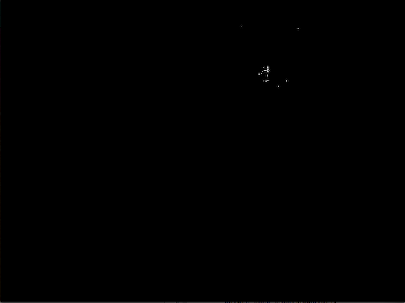
\includegraphics[scale = 0.3]{img/bad4t}
                \caption{}
        \end{subfigure}
		\quad
        \begin{subfigure}[b]{0.35\textwidth}
                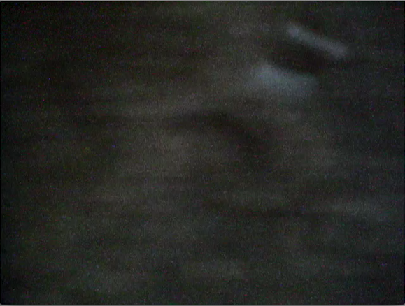
\includegraphics[scale = 0.3]{img/bad4}
                \caption{}
        \end{subfigure}
		\caption{Examples of tracking failues.}
		\label{fig:ant_fail}
\end{figure}

In image \emph{b} and \emph{d} in Figure \ref{fig:ant_fail}, the tracking fails because the ant is no longer the largest object in the thresholded images \emph{a} and \emph{c}. In image \emph{b} it is because the gound reflects too much light, and in image \emph{d} it is because the water reflects too much light. One might wonder why, especiallyin image \emph{c}, the ant is considered smaller than the reflection. This is because the blob detector in OpenCV, assume blobs are \emph{circular} and the size of a blob is actually the radius of that circle. Because the blob is lengthy but slim the radius of the circle surrounding the entire blob becomes very large, and as such the radius size reported by the blob detector as well. This leads to the problem that our software interprets the water reflection to be the largest blob in the image. \\

In image \emph{f} the problem arises because the images is too dark. Even with then given contrast, most of the white color does no make the threshold boundary, and the pixels that makes it past the thresold is considered noise by the blob detector. In image \emph{d} the image is simply too blurry (the ant is in the upper left corner), which makes both the ant and the white color "disappear" into the background.\\

In summary the problems throughout our test can be generalized to cover the following issues:

\begin{itemize}
    \item Background reflections
    \item Bad lighting of test area
    \item Camera blurryness
    \item Ant speed
\end{itemize}

To solve the issues of background reflections and light conditions a lab environment could be established were there would be no daylight involved, and have the entire test area be lit by diffuse light. This would ensure both a much better lit ant, and possibly also a solution to track an ant using other colors than white. Furthermore, reflections would not be as apparant due to the lack of a strong single light source, and would further reduce shadows from the arm of the plotter moving the camera around.\\

During the test it was noticed that the ants we had available in general moved very fast, and every so often they would move out of the cameras view in a second or two. But most of the time the camera could keep up with the ant, but because of the speed many of the images produced by the camera were very blurry, and at some point tracking would fail because the ant could no be located in the blurry images as shown in Figure \ref{fig:ant_fail}. To solve this issue, one could use ants that moved slower, or move the camera further up from the ground, such that it did not have to move as much between every frame as in our case. We do not know if termites moves as fast as the ants we have available, and if not, then they would be easier to monitor and follow with this setup. We also noticed during the test that the increased speed of the ants were often triggered when they were frigthened. We noticed this when we caught ants to be painted, and when released ants into the test environment. Over time they would slow down when they became relaxed (or so we assume). During our test, the old XY-plotter would stutter from time to time, making large noises and shake the petri dish for a few seconds, and this probably caused a frightened reaction with the ant, seing as it started to move very fast again, escaping the camera due to blurry images. With newer and more robust hardware this could be avoided. It should be noted that putting the ants in a freezer for a couple of minutes would paralyze them, and until fully recovered, they would move much slower, greatly improving the tracking capabilities.\\

Another observation about the test is that the ant itself were almost never visible in the images (atleast not to the human eye) and completely disappearing in blurry images, where the white color would still be visible. It is worth noting that this would really complicate tracking of \emph{multiple ants} if the others are not painted as well. This would also complicate the solution further as the software would need to account for multiple colors at the same time, however with a proper lit lab environment this would be doable.\\

In conclusion, we argue that the software itself works as intended, with only a few situations where it is the cause of the failed tracking. The failed tracking can mostly be credited to a poor test setup, test environment, hardware difficulties and the animals themselves moving much faster than anticipated before the test.\\
